%
\hsection{\crowsFoot{S}{MM}{T}{MM}}%
\label{sec:rm:st}%
%
\begin{figure}%
\centering%
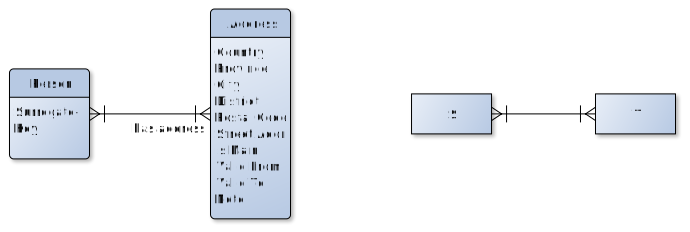
\includegraphics[width=0.97\linewidth]{\currentDir/ST}%
\caption{We encountered the \crowsFoot{S}{MM}{T}{MM} relationship pattern in \cref{fig:erdPlatform1}.}%
\label{fig:rm:st}%
\end{figure}%
%
\gitSQLAndOutput{\databasesCodeRepo}{conceptualToRelational}{ST_tables.sql}{relationships}{}{}{postgres.sh}{ST_tables}{%
The realization of a \crowsFoot{S}{MM}{T}{MM} conceptual relationship.%
}%
\gitSQLAndOutput{\databasesCodeRepo}{conceptualToRelational}{ST_insert_and_select.sql}{relationships}{}{}{postgres.sh}{ST_insert_and_select}{%
Inserting into and selecting data from the realization of an \crowsFoot{S}{MM}{T}{MM} conceptual relationship given in \cref{lst:ST_tables}.%
}%
%
\gitExecPath{\databasesCodeRepo}{conceptualToRelational}{../_scripts_/db_table_to_latex_table.sh relationships s sid;fktid;x}{cdtrmTableS}%
\gitExecPath{\databasesCodeRepo}{conceptualToRelational}{../_scripts_/db_table_to_latex_table.sh relationships t tid;fksid;y}{cdtrmTableT}%
\gitExecPath{\databasesCodeRepo}{conceptualToRelational}{../_scripts_/db_table_to_latex_table.sh relationships relate_s_and_t fksid;fktid}{cdtrmTableRST}%
%
\begin{figure}%
\centering%
\floatSep%
\input{\cdtrmTableS}%
\floatSep%
\input{\cdtrmTableT}%
\floatSep%
\input{\cdtrmTableRST}%
\floatSep%
\caption{The contents of the the three tables in the implementation of the \crowsFoot{S}{MM}{T}{MM} conceptual relationship after executing \cref{lst:ST_insert_and_select}.}%
\label{fig:rm:st:tables}%
\end{figure}%
%
\gitSQLAndOutput{\databasesCodeRepo}{conceptualToRelational}{ST_insert_error_1.sql}{relationships}{}{}{postgres.sh}{ST_insert_error_1}{%
Trying to insert new related rows into tables~\sqlil{s} and~\sqlil{t} without updating table~\sqlil{relate_s_and_t} does not work.%
}%
\gitSQLAndOutput{\databasesCodeRepo}{conceptualToRelational}{ST_insert_error_2.sql}{relationships}{}{}{postgres.sh}{ST_insert_error_2}{%
Trying to insert a new row into tables~\sqlil{s} and relate it to an existing row in table~\sqlil{t} without updating table~\sqlil{relate_s_and_t} does not work either.%
}%
%
We have the two entity types~S and~T.
Each entity of type~S must be connected to at least one entity of type~T, but can be connected to many.
Each entity of type~T must be connected to at least one entity of type~P, but can be connected to many.

We encountered this relationship pattern back in \cref{fig:erdPlatform1} when constructing the overall model of our teaching management platform.
Back then, we related address records to person entities.
Each person must have at least one address, but may have more than one address.
Each address stored in our system must be associated with at least one person, but it is possible that multiple people live at the same place.
This part of the model is sketched in \cref{fig:rm:st}.

To implement this relationship pattern, we will combine what we learned when implementing the \crowsFoot{M}{M1}{N}{MM}~pattern in \cref{sec:rm:mn} with the method for implementing the \crowsFoot{Q}{OM}{R}{MM}~pattern in \cref{sec:rm:qr}.

We first again create the basic tables that we are definitely going to need in \cref{lst:ST_tables}.
We need a table~\sqlil{s} for the entities of type~S.
The primary key of this table be~\sqlil{sid} and there also will be the example attribute~\sqlil{x}.
We also need a table~\sqlil{t} for the entities of type~T, which gets the primary key~\sqlil{tid} and the example attribute~\sqlil{y}.%
%
\begin{sloppypar}%
We will also definitely need a third table to manage the relationships, which we will call~\sqlil{relate_s_and_t}.
This table has two columns,~\sqlil{fksid} and~\sqlil{fktid}, which are foreign keys pointing to the primary keys~\sqlil{sid} and~\sqlil{tid} of tables~\sqlil{s} and~\sqlil{t}, respectively.
This is ensured with corresponding \sqlil{REFERENCES} constraints.
Both columns also are marked as~\sqlil{NOT NULL}, because neither value can be omitted in a row.
Like in \cref{sec:rm:op}, each pair~\sqlil{(fksid, fktid)} can appear only once in the table, because two specific rows in tables~\sqlil{s} and~\sqlil{t} can, of course, be related only once to each other.
This is implemented via the constraint~\sqlil{PRIMARY KEY (fksid, fktid)}.%
\end{sloppypar}%
%
Like in the \crowsFoot{M}{M1}{N}{MM}~pattern, both relationship ends are mandatory.
We cannot create a row in table~\sqlil{s} without relating it to an existing row in table~\sqlil{t}.
We also cannot create a row in table~\sqlil{t} without relating it to an existing row in table~\sqlil{s}.
Back in \cref{sec:rm:mn}, we solved this chicken-and-egg problem by creating a sequence from which we could then generate values for the primary key of the table~\sqlil{m}.
We would use this sequence to first create a primary key, use the primary key as foreign key in the table~\sqlil{n}, and use the primary key of that row together with the one for table~\sqlil{m} to finally insert a new row in table~\sqlil{m}.
We will follow a similar approach here, so we first invoke~\sqlil{CREATE SEQUENCE sqsid AS INT;}.
The primary key for table~\sqlil{s} is then defined as~\sqlil{sid INT DEFAULT NEXTVAL('sqsid') PRIMARY KEY}.

Both tables~\sqlil{s} and~\sqlil{t} will have a column referencing a primary key from the respective other table.
For table~\sqlil{s}, this is column~\sqlil{fktid}, and for table~\sqlil{t}, this is column~\sqlil{fksid}.
These will be used to enforce that each row in table~\sqlil{s} is definitely related to one row in table~\sqlil{t} and vice versa.
Of course, they can also be related to multiple rows, which is why we need to manage the relationships in table~\sqlil{relate_s_and_t}.%
%
\begin{sloppypar}%
We also must make sure that for each row in table~\sqlil{s} with data~\sqlil{(sid, fktid)}, there exists a corresponding row~\sqlil{(fksid, fktid)} in table~\sqlil{relate_s_and_t}.
We do this by adding the constraint~\sqlil{s_sid_fktid_fk} which is~\sqlil{FOREIGN KEY (sid, fktid)} that~\sqlil{REFERENCES relate_s_and_t (fksid, fktid)} to table~\sqlil{s}.
This is the exactly same approach we used for the \crowsFoot{Q}{OM}{R}{MM}~pattern in \cref{sec:rm:qr}.%
\end{sloppypar}%
%
The difference is that we must do this also for table~\sqlil{t}, because both relationship ends are mandatory.
In other words, we add the constraint~\sqlil{t_fksid_tid_fk} to table~\sqlil{t} that ensures that every tuple~\sqlil{(fksid, tid)} in that table must also appear as tuple~\sqlil{(fksid, fktid)} in table~\sqlil{relate_s_and_t}.

Defining the constraints that enforce referential integrity for pattern is one thing, finding a way to insert data into the tables under these tight constraints is another issue.
In \cref{lst:ST_insert_and_select}, we do that.

Initially, the tables are empty.
This means that we need to create three rows at once:
We need to create a row in table~\sqlil{s} and we must immediately relate it to a newly created row in table~\sqlil{t} \emph{and} this relationship must also appear as row in table~\sqlil{relate_s_and_t}.
Thanks to \pglspl{CTE}, this is possible.

First, we create a new primary key value for table~\sqlil{s} by creating the \pgls{CTE}~\sqlil{s_id} corresponding to \sqlil{SELECT NEXTVAL('sqsid') AS new_sid}.
We then use this new primary key value when inserting a row into table~\sqlil{t} via~\sqlil{INSERT INTO t (y, fksid) SELECT 'AB', new_sid FROM s_id}.
Of course, we do this as another \pgls{CTE} named~\sqlil{new_t} also doing~\sqlil{RETURNING tid, fksid}.
This means that this \pgls{CTE} will provide is the primary key of the new row in table~\sqlil{t} and the primary key~\sqlil{fksid} that we already allocated for the row in table~\sqlil{s} that we will create next.
And now we create this row.
We invoke \sqlil{INSERT INTO s (sid, x, fktid) SELECT fksid, '123', tid FROM new_t}.
Notice how this uses the pre-created primary key as, well, primary key.
It also uses the primary key of the new row in table~\sqlil{t} as foreign key.
This is going to be our third \pgls{CTE}, called~\sqlil{new_s}, which also returns both keys via~\sqlil{RETURNING sid, fktid}.
Finally, we can insert a row into~\sqlil{relate_s_and_t} by doing \sqlil{INSERT INTO relate_s_and_t (fksid, fktid) SELECT sid, fktid FROM new_s}.
Thanks to \pglspl{CTE}, we could insert one row in three tables each, in a single \sql\ command, which performs the referential integrity checks at its end.%
%
\begin{sloppypar}%
Now there are existing records in the tables~\sqlil{s} and~\sqlil{t}.
It is comparatively easy to create a new row for table~\sqlil{s} that is related to an existing row in table~\sqlil{t}.
In this case, all we need to do is to insert the row into table~\sqlil{s} and, at the same time, insert a row into table~\sqlil{relate_s_and_t}.
We just need a single~\pgls{CTE}, which we will call~\sqlil{new_s}, and which performs \sqlil{INSERT INTO s (x, fktid) VALUES ('456', 1) RETURNING sid, fktid}.
As result, we get the primary key~\sqlil{sid} of the new row in table~\sqlil{s} as well as the foreign key to table~\sqlil{t}, \sqlil{fktid}, which is the same as the one we provided when creating the row in table~\sqlil{s}, namely~\sqlil{1}.
We can then \sqlil{INSERT INTO relate_s_and_t (fksid, fktid) SELECT sid, fktid FROM new_s} and are done.%
\end{sloppypar}%
%
\begin{sloppypar}%
Since the relationship pattern is symmetric, we can do exactly the same for table~\sqlil{t}.
We can insert a new row into table~\sqlil{t} and relate it to an existing row in table~\sqlil{s}.
For this, we would proceed the same way and also use one~\pgls{CTE}.
Finally, we can also simply relate two existing rows in tables~\sqlil{s} and~\sqlil{t} by just creating one new row in table~\sqlil{relate_s_and_t}.
This can be like this:~\sqlil{INSERT INTO relate_s_and_t VALUES (1, 3);}.
The contents of all three tables after inserting the data are shown in \cref{fig:rm:st:tables}.%
\end{sloppypar}%
%
Merging the data requires again two \sqlil{INNER JOIN} expressions, exactly as before.
The constraints prevent us from creating rows in~\sqlil{s}~(or~\sqlil{t}) that are not related to rows in~\sqlil{t}~(or~\sqlil{s}).
We also cannot relate rows without creating the corresponding entry in~\sqlil{relate_s_and_t}, as shown in \cref{lst:ST_insert_error_1,lst:ST_insert_error_2}.%
%
\FloatBarrier%
\endhsection%
%
